\subsection{Performance comparison with iZ3 and MathSat}\label{performance_oct}

This section discusses a parametrized problem 
in the UTVPI theory and compares the times required by
our implementation, iZ3, and Mathsat.

\begin{lemma} \label{performance_test_lemma_oct}
  Let $x_i$ for $1 \leq i \leq n$ where $n \in \mathbb{N}$ is fixed.
  The following conjunction of inequalities is unsatisfiable:
  \begin{equation*}\label{oct_problem}
    x_1 + x_2 \leq 1 
    \land \bigwedge_{i=2}^{n-1} (x_{i+1} - x_i \leq 1) 
    \land x_1 - x_n \leq 1
    \land x_1 > \ceil{n/2}
  \end{equation*}
\end{lemma}

\begin{proof}
  Using the inequalities $x_1 + x_2 \leq 1 
  \land \bigwedge_{i=2}^{n-1} (x_{i+1} - x_i \leq 1)$
  we can conclude that $2x_1 \leq n$.
  The latter contradicts the last inequality $x_1 > \ceil{n/2}$.
\end{proof}

The interpolation pair for our performance test 
is $(x_1 + x_2 \leq 1 
  \land \bigwedge_{i=2}^{n-1} (x_{i+1} - x_i \leq 1) 
\land x_1 - x_n \leq 1, x_1 > \ceil{n/2})$
for fixed $n \in \mathbb{N}$.
It is easy to see that the pair is inconsistent due to the lemma 
\ref{performance_test_lemma_oct}. 

By lemma \ref{performance_test_lemma_oct}
we can also see that the formula $x_1 \leq \ceil{n/2}$ is an 
interpolating formula for all fixed $n$ in this parametrized problem.
Similarly to the parametric problem in \ref{performance_euf}, 
we designed this problem because it is easy to verify the 
correctness of output of the algorithms and to measure 
the time for various values of $n$. 
We executed instances of this problem for values of $n$
in the range $\{1, \dots, 10000\}$ using the same setup 
used in the performance comparison for the parametrized 
problem discussed in \ref{performance_test_lemma}.
The follow graph shows similar results as 
in \ref{performance_test_lemma}.

\begin{figure}
  \centering
  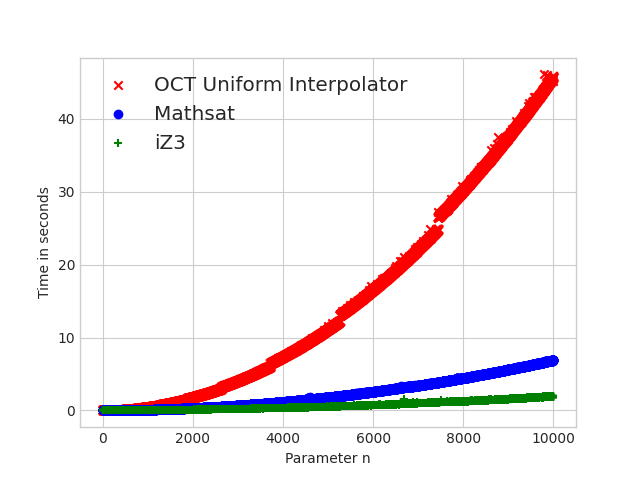
\includegraphics[scale=0.9]{figures/octi_performance_graph}
  \caption{Performance comparison graph of Oct interpolant generation
  algorithms for paramatrized problem from section \ref{performance_oct}} 
  \label{performance_graph_euf}
\end{figure}

We noticed a quadractic behaviour in the graph for the time 
required by all the algorithms. Indeed, the latter was
validated since a quadratic fitting has a smaller quadratic
error compared to a linear fitting in all the implementations
as show in the following table:

\begin{table}[h]
  \centering
  \begin{tabular}{ccc}
    \toprule
    {}                 & Error of linear fitting & Error of quadratic fitting \\
    \cmidrule{2-2} \cmidrule{3-3}                                             \\
    iZ3                & 3.2311742677852644e-25 & 1.269128969536517e-23       \\
    Mathsat            & 2.3207586060940883e-22 & 1.1983240884566356e-22      \\
    Our implementation & 2.9778502051908996e-21 & 1.455131710005814e-20       \\
    \bottomrule
  \end{tabular}
  \caption{Table of polynomial fitting errors of degrees 1, 2 for the
  Octagon experiments of section \ref{performance_oct}.}
\end{table}

%%% Local Variables:
%%% mode: latex
%%% TeX-master: "main"
%%% End:
